\chapter{PROBLEM 2}
\begin{center}\large\bfseries CONCURRENCY, AVAILABILITY, \& GRACEFUL DEGRADATION\end{center}

\section{Rancangan Solusi dan Mekanisme}
P2 memeriksa apakah sumber yang lambat atau gagal ikut menghambat layanan lain. Rancangan memisahkan pekerjaan polling dari request client, memberi jalur baca kapasitas tersendiri, dan tetap menyajikan data terakhir ketika sumber mengalami outage. Metadata freshness membantu client menilai kondisi data yang diterima.

\subsection{Isolasi request dan polling}
Jalur request client dipisahkan dari pengambilan data sumber. Client API membaca data yang telah tersimpan melalui Aggregator, sehingga request tidak harus menunggu mock PVMBG yang dapat terlambat 3 detik. Sementara itu, loop polling BMKG dan PVMBG berjalan sendiri-sendiri; fetch seismic dan warning BMKG juga dapat dilakukan paralel. HTTP client menggunakan kembali koneksi untuk mengurangi biaya pembukaan koneksi pada request berikutnya.

Di database, pekerjaan baca memiliki pool 10 koneksi, sedangkan penulisan BMKG, penulisan PVMBG, dan relay masing-masing mendapat 2 koneksi. Dengan pemisahan ini, pekerjaan polling tidak mengambil seluruh koneksi yang dibutuhkan jalur baca. API dan Aggregator membatasi jumlah request yang sedang diproses menjadi 128. Jika batas tersebut tercapai, service mengembalikan 429 beserta \texttt{Retry-After}, sehingga client mengetahui bahwa request perlu dicoba lagi.

Timeout membatasi lamanya setiap pekerjaan: baca database 200 ms, write 2 detik, request API ke Aggregator 1 detik, request ke BMKG 1 detik, dan request ke PVMBG 4 detik. Angka PVMBG dibuat lebih panjang agar delay 3 detik pada pengujian masih dapat ditangani.

\subsection{Degradasi dan pemulihan sumber}
Kegagalan sumber tidak selalu berarti data tidak dapat disajikan. Ketika polling PVMBG gagal, Aggregator mempertahankan record terakhir yang berhasil disimpan. API masih mengembalikannya, tetapi \texttt{meta.sources.PVMBG.status} menjadi \texttt{stale} untuk menunjukkan bahwa pembaruan sumber terganggu. Respons menyertakan \texttt{last\_success\_at} dan \texttt{stale\_since} sebagai penanda waktu. BMKG dapat tetap \texttt{fresh} karena polling-nya berjalan terpisah.

Status \texttt{unavailable} digunakan jika sumber belum mempunyai poll yang berhasil penuh maupun record valid yang tersimpan. Jika polling pertama hanya berhasil sebagian, record valid tetap dapat dibaca dengan status stale; \texttt{last\_success\_at} tetap null sampai satu siklus berhasil penuh. Dengan aturan ini, kegagalan satu record tidak menyembunyikan record lain yang sudah tersimpan.

Untuk pembacaan daftar, status HTTP mengikuti ketersediaan sumber yang diminta. API mengembalikan 503 dengan kode \texttt{SOURCE\_UNAVAILABLE} jika seluruh sumber yang diminta belum tersedia. Request khusus PVMBG akan memperoleh 503 pada kondisi tersebut, sedangkan request gabungan tetap dapat memperoleh 200 berisi data BMKG jika BMKG tersedia. Metadata tetap menyatakan PVMBG unavailable, sehingga respons gabungan tidak memberi kesan bahwa kedua sumber tersedia.

Setelah outage dinonaktifkan, polling berikutnya memperbarui data dan mengembalikan PVMBG menjadi fresh tanpa restart API atau Aggregator. Selain kegagalan polling, data juga dianggap stale jika waktu sukses terakhir telah melewati ambang 15 detik pada konfigurasi awal.

\section{Alasan Keputusan dan Trade-off}
Alternatifnya adalah mengambil data sumber untuk setiap request client. Cara itu dapat memberikan data yang lebih baru, tetapi waktu respons dan kegagalan sumber langsung memengaruhi client. Polling menghindari ketergantungan tersebut dengan konsekuensi adanya jeda pembaruan. Karena itu, API menyertakan metadata freshness agar client mengetahui status sumber dan waktu pembaruan terakhir.

Pool koneksi dan batas request dipilih agar pekerjaan yang lambat tidak menghabiskan seluruh resource. Satu pool bersama lebih sederhana dikonfigurasi, tetapi writer sumber dan request baca akan berebut kapasitas yang sama. Pemisahan pool memberi jalur baca kapasitas tersendiri, dengan konsekuensi total koneksi database harus diperhitungkan. Batas request dan timeout juga dapat menolak atau menghentikan pekerjaan saat beban tinggi, tetapi mencegah antrean tumbuh tanpa batas.

\section{Batasan yang Disadari}
Hasil load test menggambarkan beban yang dicoba pada satu host dengan pembacaan maksimal 50 record per request. Pengujian tersebut ditujukan untuk memeriksa ambang beban pada spesifikasi, sehingga belum mencari kapasitas maksimum sistem. Jalur baca tetap membutuhkan Aggregator dan PostgreSQL. Keduanya belum memiliki failover karena deployment M1 memakai satu instance per komponen; isolasi dari gangguan sumber karena itu tidak menjamin API tersedia jika salah satu komponen ini mati.

Penilaian freshness masih menggunakan wall clock. Jika waktu host bergeser, umur data yang ditampilkan dapat ikut berubah meskipun pengukuran latency tetap benar. Perluasan ke beberapa node karena itu memerlukan sinkronisasi waktu serta pengujian ulang terhadap kapasitas dan pola kegagalan yang baru.

\section{Bukti Penyelesaian}
Pengujian P2 mencakup outage dan pemulihan sumber, serta load test dengan delay PVMBG 3 detik. Hasilnya ditunjukkan melalui command outage dan berkas pengukuran berikut [10].

Penanganan record valid dari poll parsial juga diperiksa melalui uji regresi \texttt{availability\_integration\_test.go} pada commit \texttt{e94e03b}. Uji dengan PostgreSQL ini mencakup BMKG dan PVMBG: data parsial dapat dibaca dengan status stale, sedangkan sumber tanpa record valid tetap menghasilkan 503.

\subsection{Outage dan pemulihan}
Pengujian outage dilakukan melalui endpoint kontrol mock. Request berikut mengirim \texttt{enabled=true} ke \texttt{/admin/outage}; setelah respons diterima, pengujian menunggu polling mendeteksi kegagalan sumber.
\terminalfigure{p2-outage-control}{Mengaktifkan outage pada sumber PVMBG.}{fig:p2-outage-control}

Berikutnya, dua request dikirim ke Client API dengan token Tim Lapangan. Request pertama memilih PVMBG dan menampilkan jumlah record beserta metadata sumber, sedangkan request kedua membaca metadata BMKG. Hasilnya menunjukkan lima record PVMBG masih dapat dibaca, dengan status stale dan waktu kegagalan yang tercatat. Pada saat yang sama, BMKG tetap fresh. Dengan demikian, outage PVMBG tidak menghilangkan data terakhir atau mengganggu status pembaruan BMKG.
\terminalfigure{p2-outage}{Respons API selama PVMBG outage: data terakhir tersedia dan kondisi setiap sumber dinyatakan secara eksplisit.}{fig:p2-outage}

Pemulihan dilakukan dengan mengirim \texttt{enabled=false} ke endpoint yang sama. Setelah jeda polling, request API menunjukkan PVMBG kembali fresh dan \texttt{stale\_since} menjadi null. Langkah ini tidak menjalankan command restart. Trial integrasi juga membandingkan kondisi container sebelum dan sesudah outage; hasilnya tersimpan di \texttt{outage-recovery.json}.
\terminalfigure{p2-recovery}{Mematikan outage dan membaca hasil polling yang sudah pulih.}{fig:p2-recovery}

\subsection{Metode dan hasil load test}
\label{sec:p2-load}
Load test mengukur respons API ketika kedua jenis data dibaca bersamaan dan sumber PVMBG diberi delay. Pengujian menggunakan \path{scripts/load/hazards-monotonic.py}, dengan 30 worker BMKG dan 30 worker PVMBG selama 90 detik. Setiap worker langsung mengirim request berikutnya setelah menerima respons, tanpa think time.

Setiap worker mempunyai sesi Tim Lapangan sendiri, menggunakan HTTP keep-alive, dan membaca \texttt{view=full} dengan limit 50. Access token tetap menggunakan TTL 60 detik; script melakukan refresh sebelum expiry agar masa berlaku token tidak menjadi penyebab putusnya beban. Selama pengujian, delay sumber PVMBG ditetapkan 3000 ms.

Latency dihitung sejak request dimulai hingga seluruh body diterima, termasuk pembukaan koneksi jika diperlukan. Pengukuran memakai \path{time.perf_counter_ns}, yaitu timer monotonic yang tidak mengikuti perubahan wall clock host, sedangkan percentile dihitung dengan metode nearest rank.

Untuk memeriksa syarat koneksi paralel, collector menggunakan Linux \texttt{ss} dan mengambil sampel koneksi TCP established ke port API setiap sekitar 1 detik. Pengukuran ini diperlukan karena jumlah worker saja tidak membuktikan jumlah koneksi yang benar-benar terbuka.

Sebelum beban diberikan, delay mock diatur dengan body \texttt{min\_ms} dan \texttt{max\_ms} yang sama-sama bernilai 3000. Request langsung ke sumber kemudian mengukur waktu respons melalui \texttt{curl}. Flag \texttt{-o /dev/null} membuang body, sedangkan \texttt{-w} menampilkan status HTTP dan durasi request. Pengukuran ini membedakan delay sumber dari latency Client API yang membaca data tersimpan.
\terminalfigure{p2-delay}{Mengatur delay 3 detik dan mengukur request langsung ke sumber PVMBG.}{fig:p2-delay}

Collector TCP dijalankan bersamaan dengan load test untuk mengukur jumlah koneksi established selama beban berlangsung. Kedua proses dimulai dari root repo dengan command berikut:
\begin{lstlisting}
export API_URL=http://127.0.0.1:8280
export AUTH_URL=http://127.0.0.1:8284
python3 scripts/load/capture-tcp-connections.py \
  --api-url "$API_URL" --seconds 110 --interval 1 \
  --output /tmp/report-tcp.json &
tcp_pid=$!
python3 scripts/load/hazards-monotonic.py \
  --seconds 90 --vus-per-source 30 --output /tmp/report-load.json
wait "$tcp_pid"
\end{lstlisting}
Hasil load test tersimpan di \path{docs/report/evidence/load.json}. Field yang diperiksa meliputi jumlah worker, durasi pengujian, p95 BMKG, throughput, dan persentase error.
\terminalfigure{p2-load}{Membaca hasil load test dari berkas pengukuran yang disimpan.}{fig:p2-load}

\begin{table}[H]
\centering\small
\begin{tabular}{lrr}
\toprule
Metrik & BMKG & PVMBG \\
\midrule
Request terkirim & 44.510 & 43.828 \\
Respons sukses & 44.494 & 43.814 \\
Error selain 429 & 16 & 14 \\
HTTP 429 pada API & 0 & 0 \\
p50 sukses (ms) & 52,07 & 52,64 \\
p95 sukses (ms) & 124,52 & 125,24 \\
p99 sukses (ms) & 190,71 & 194,30 \\
p95 seluruh respons (ms) & 124,76 & 125,44 \\
\bottomrule
\end{tabular}
\caption{Hasil beban simultan selama 90,09 detik. p50/p95/p99 sukses dihitung dari 2xx; p95 seluruh respons juga ditampilkan.}
\label{tab:load}
\end{table}
Dari 88.338 request yang dikirim, 88.308 mendapat respons sukses. Throughput-nya mencapai 980,26 respons sukses per detik, sedangkan 30 request lainnya menghasilkan HTTP 503, sebagaimana dicatat dalam \path{docs/report/evidence/load-statuses.json}. Dengan demikian, error selain 429 sebesar 0,034\%, masih di bawah batas 1\%.

API tidak menghasilkan 429, sedangkan Auth menghasilkan 18 respons 429 selama login dan refresh. Retry berhasil sehingga seluruh sesi worker tetap berjalan. Respons Auth dicatat terpisah dari error pembacaan hazard.

Delay PVMBG terukur 3.004,46 ms, sedangkan p95 BMKG 124,52 ms memenuhi batas 300 ms saat kedua sumber dibaca bersamaan. Collector mencatat sedikitnya 50 koneksi pada rangkaian sampel selama 89,00 detik, melebihi syarat 60 detik. Pengambilan sampel sekitar sekali per detik menentukan resolusi bukti koneksi tersebut.

\begin{figure}[H]
\centering
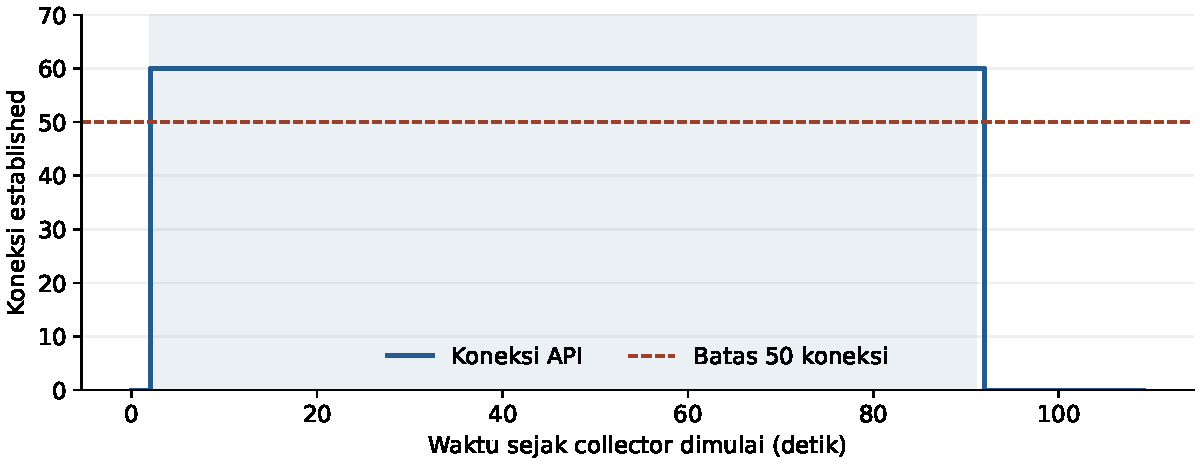
\includegraphics[width=\textwidth]{figures/p2-tcp.pdf}
\caption{Sampel koneksi established selama pengujian. Garis putus-putus menunjukkan batas 50 koneksi. Interval di atas batas dihitung dari rangkaian sampel koneksi.}
\label{fig:p2-tcp}
\end{figure}

\begin{table}[H]
\centering\small
\begin{tabularx}{\textwidth}{>{\raggedright\arraybackslash}p{2cm}Y}
\toprule
Kriteria & Bukti \\
\midrule
P2.1 & Delay sumber terukur dan BMKG p95 pada Tabel~\ref{tab:load}; kedua sumber menerima request bersamaan. \\
P2.2 & Throughput, percentile, error, 429, serta sampel TCP; Tabel~\ref{tab:load} dan Gambar~\ref{fig:p2-tcp}. \\
P2.3 & Kontrol outage, data stale, dan pemulihan pada Gambar~\ref{fig:p2-outage-control}--\ref{fig:p2-recovery}; trial lengkap di \texttt{outage-recovery.json}. \\
P2.4 & Model konkurensi dan penanganan tiga kegagalan pada Bagian~\ref{sec:p2-di-laporan}; metode, command, dan hasil load test pada bagian bukti. \\
\bottomrule
\end{tabularx}
\end{table}

\begin{samepage}
\section{Jawaban atas Butir ``Di laporan''}
\label{sec:p2-di-laporan}
Model konkurensi menggunakan handler HTTP Go untuk request client dan loop polling terpisah untuk BMKG serta PVMBG. Tiga kegagalan pada P2 ditangani sebagai berikut:
\begin{enumerate}
\item \textbf{Head-of-line blocking}: request membaca Canonical Store, bukan menunggu fetch sumber. Polling PVMBG yang lambat juga tidak menahan loop BMKG.
\item \textbf{Resource exhaustion}: pool baca dipisahkan dari writer dan relay, jumlah request aktif dibatasi 128, dan setiap operasi memiliki timeout. Request di luar kapasitas ditolak secara terkendali dengan 429.
\item \textbf{Ketiadaan degradasi terkendali}: data tersimpan tetap disajikan dengan penanda stale. Sumber tanpa data dinyatakan unavailable, dan polling memulihkan freshness setelah sumber pulih.
\end{enumerate}

Load test menggunakan 30 worker per sumber selama 90 detik, HTTP keep-alive, limit 50, dan delay PVMBG 3 detik. Latency diukur dengan timer monotonic dan koneksi TCP diperiksa melalui \texttt{ss}. Tool serta command tersedia pada Bagian~\ref{sec:p2-load}; hasilnya pada Tabel~\ref{tab:load} dan Gambar~\ref{fig:p2-tcp}.
\end{samepage}
